\subsection{DAQ live rate and trigger efficiency} \label{sec:trigger}

\begin{figure}[htbp]
  \centering
  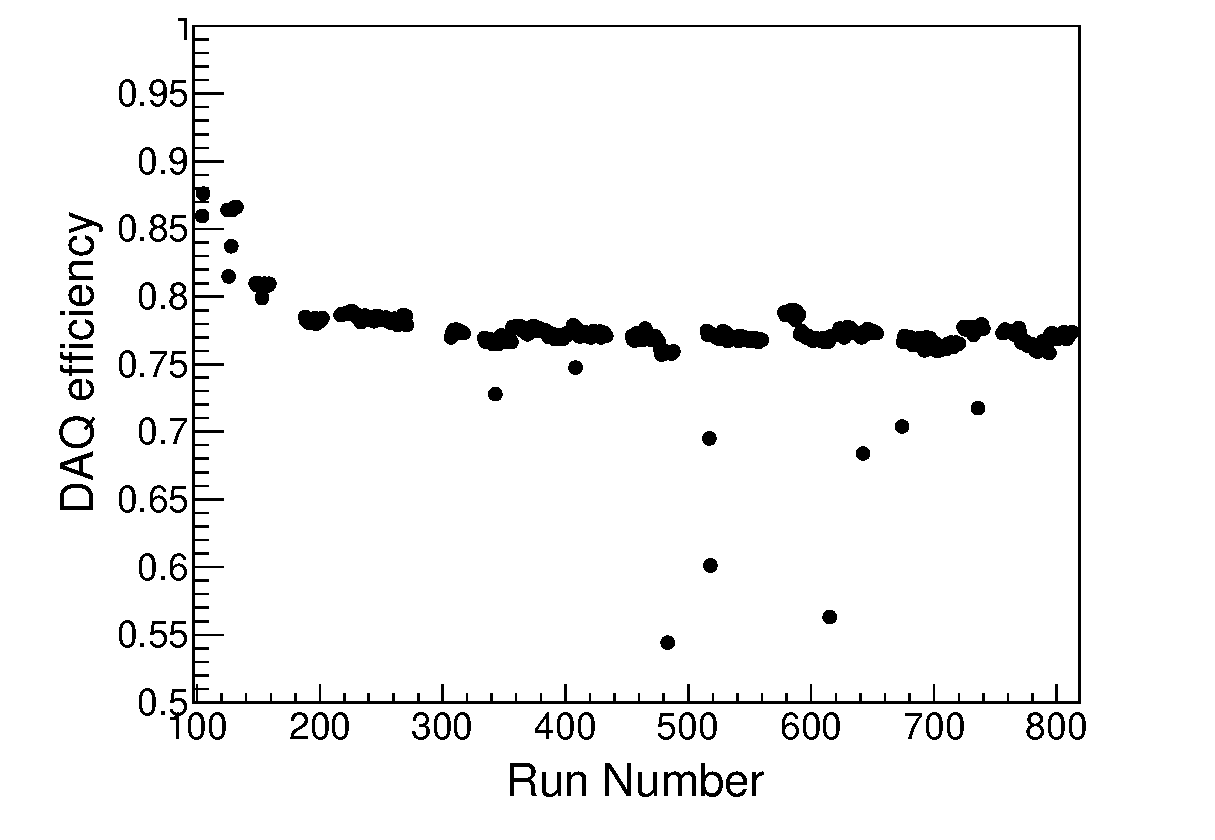
\includegraphics[width=8cm]{../pic/Run78/trigger/DAQ.eps}
  \caption{
    This figure shows DAQ live rate of production run in MR-RUN79.
  }
  \label{fig:DAQ}
\end{figure}

\begin{figure}[htbp]
  \centering
  \begin{tabular}{cc}
    \begin{minipage}{0.5\hsize}
      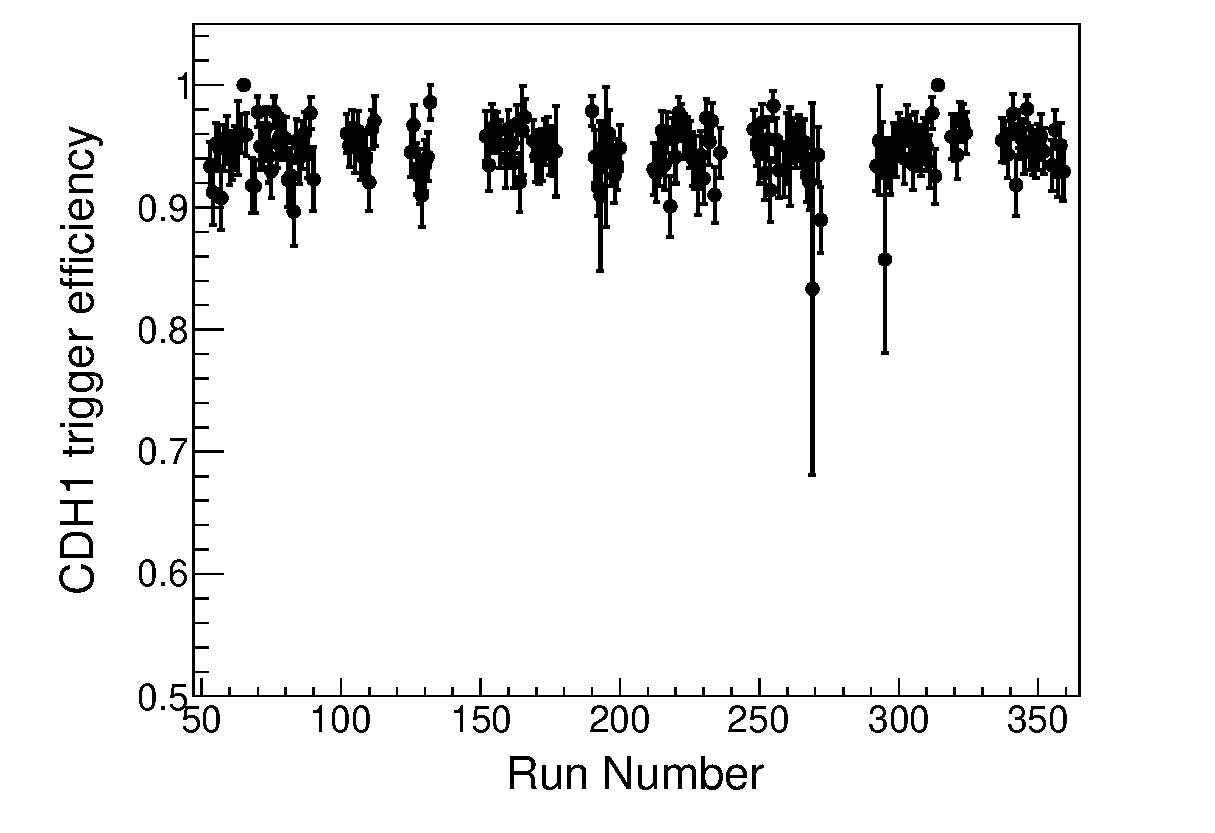
\includegraphics[width=5cm]{../pic/Run68/trigger/CDH1.eps}
    \end{minipage}

    \begin{minipage}{0.5\hsize}
      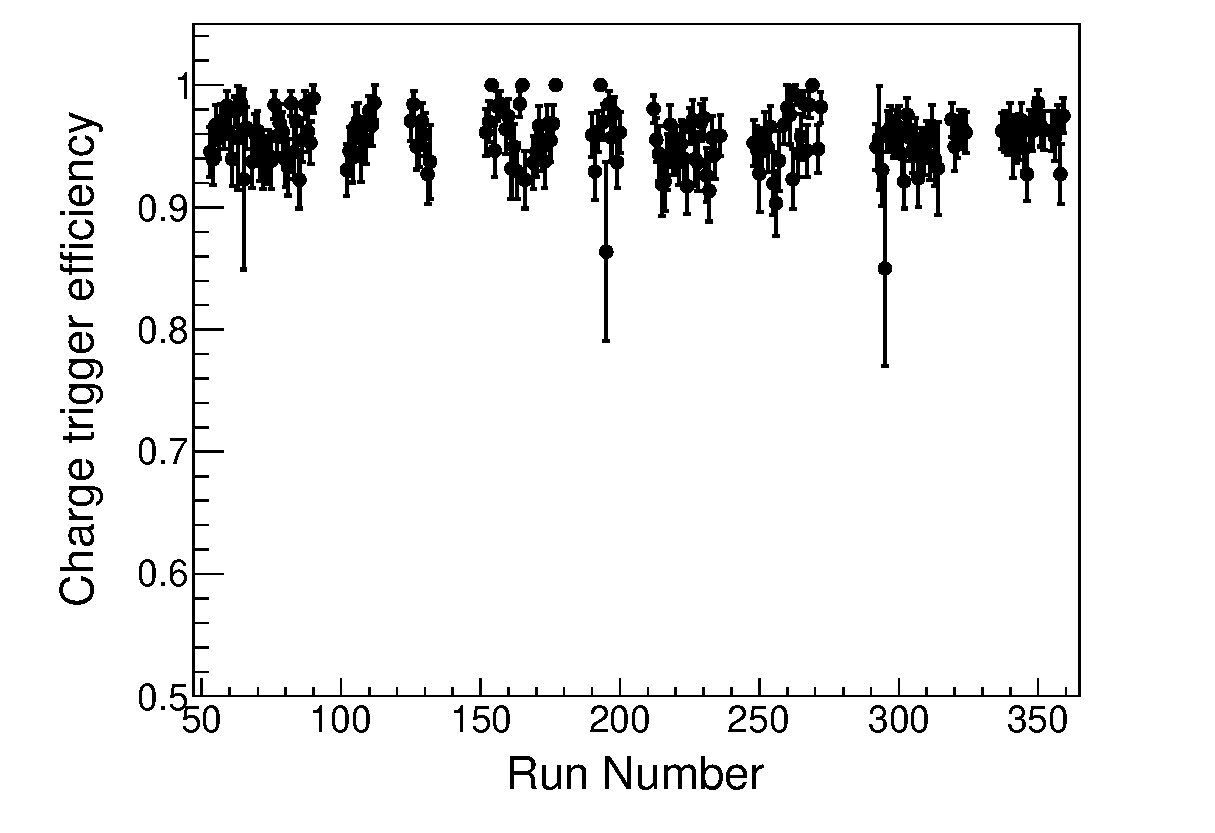
\includegraphics[width=5cm]{../pic/Run68/trigger/Charge.eps}
    \end{minipage}
  \end{tabular}

  \begin{tabular}{cc}
    \begin{minipage}{0.5\hsize}
      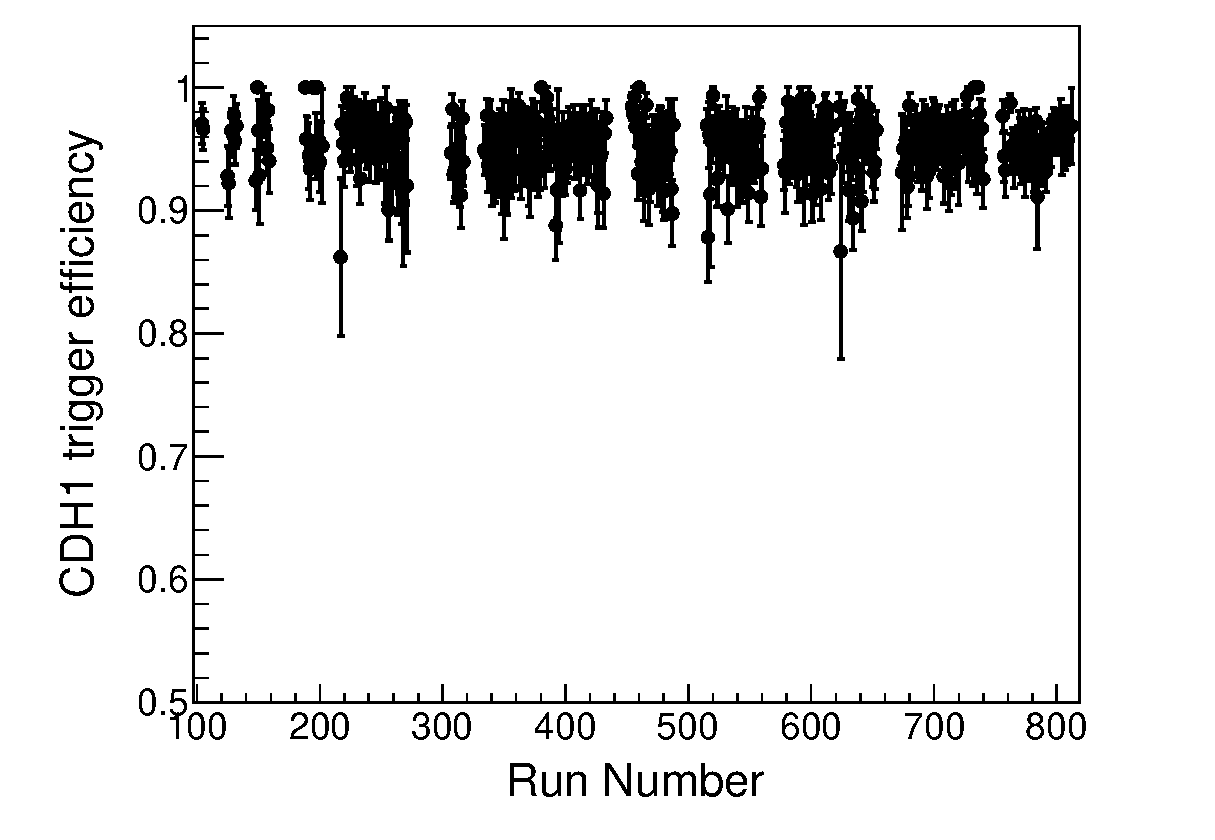
\includegraphics[width=5cm]{../pic/Run78/trigger/CDH1.eps}
    \end{minipage}

    \begin{minipage}{0.5\hsize}
      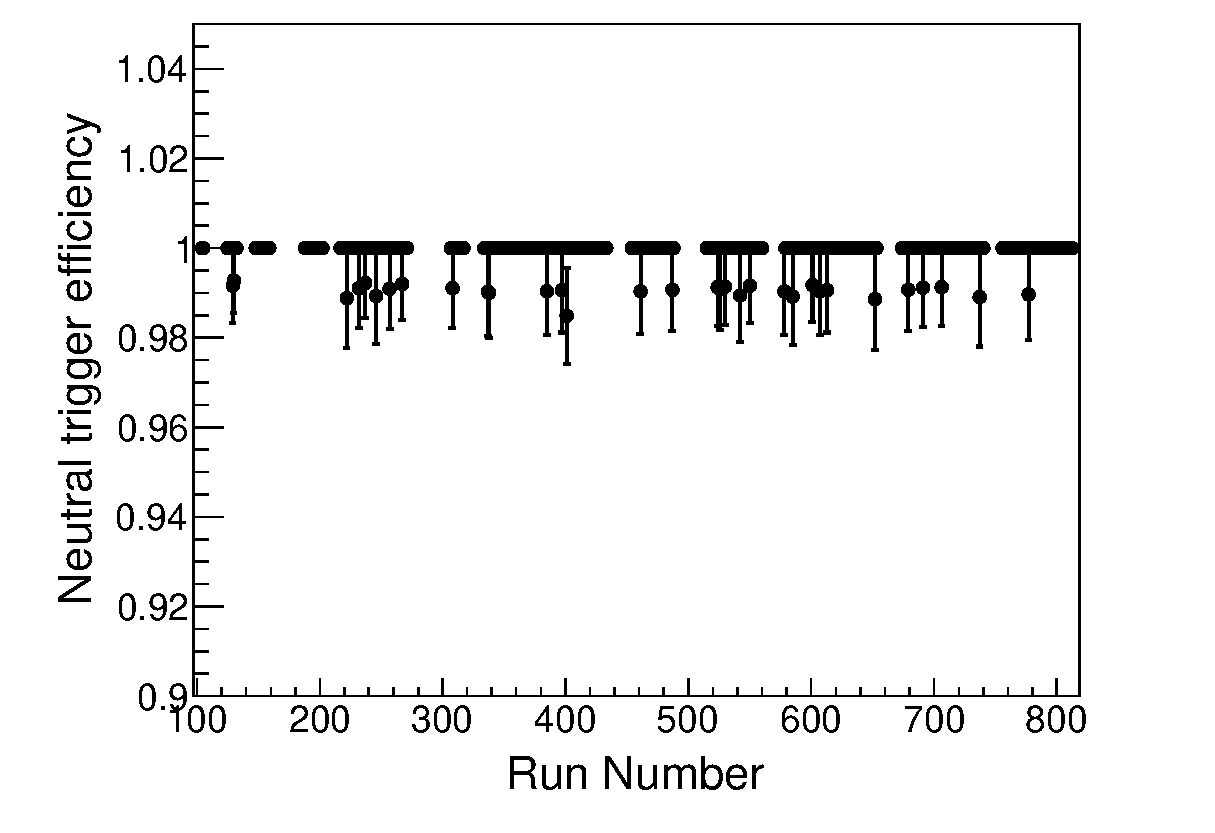
\includegraphics[width=5cm]{../pic/Run78/trigger/Neutral.eps}
    \end{minipage}
  \end{tabular}
 \caption{
    These figures show about trigger efficiencies in each run.
    The above figure represents MR-RUN69 used in the $d(K^-, p)$ analysis.
    The left figure shows the K $\otimes$ CHD1 trigger and the right figure shows the charge trigger.
    The bottom figure represents MR-RUN78 used in the $d(K^-, n)$ analysis.
    The left figure shows the K $\otimes$ CHD1 trigger and the right figure shows the neutral trigger.
  }
  \label{fig:trigger}
\end{figure}

The DAQ live ratio was evaluated by the ratio of the number of accepted events to the number of 1st trigger requests.
For MR-RUN78, these values for all runs are plotted in Figure.\ref{fig:DAQ}.

$d(K^-, n)$ and $d(K^-, p)$ trigger efficiencies were evaluated by the offline analysis in which trigger decomposed two-step.
The first part is K$\otimes$CDH1 which was estimated using unbiased Kaon trigger.
The second part is neutral$=$NC$\otimes \overline{\mbox{CVC} \otimes \mbox{BVC}}$ or charge$=$PC$\cup$CVC$_{\mbox{half}}$ which was estimated using the unbiased K$\otimes$CDH1 trigger.
Figure.\ref{fig:trigger} shows about trigger efficiency.

% These two values were evaluated run-by-run and summed up as luminosity with irradiated kaon number which is described in section.\ref{sec:kaon_num}.

